\documentclass[a4paper,norsk, 10pt]{article}
\usepackage[utf8]{inputenc}
\usepackage{verbatim}
\usepackage{listings}
\usepackage{graphicx}
\usepackage[norsk]{babel}
\usepackage{a4wide}
\usepackage{color}
\usepackage{amsmath}
\usepackage{float}
\usepackage{amssymb}
\usepackage[dvips]{epsfig}
\usepackage[toc,page]{appendix}
\usepackage[T1]{fontenc}
\usepackage{cite} % [2,3,4] --> [2--4]
\usepackage{shadow}
\usepackage{hyperref}
\usepackage{titling}
\usepackage{marvosym }
\usepackage{subcaption}
\usepackage[noabbrev]{cleveref}
\usepackage{cite}


\setlength{\droptitle}{-10em}   % This is your set screw

\setcounter{tocdepth}{2}

\numberwithin{equation}{section}

\lstset{language=c++}
\lstset{alsolanguage=[90]Fortran}
\lstset{alsolanguage=Python}
\lstset{basicstyle=\small}
\lstset{backgroundcolor=\color{white}}
\lstset{frame=single}
\lstset{stringstyle=\ttfamily}
\lstset{keywordstyle=\color{red}\bfseries}
\lstset{commentstyle=\itshape\color{blue}}
\lstset{showspaces=false}
\lstset{showstringspaces=false}
\lstset{showtabs=false}
\lstset{breaklines}
\title{FYS2140}
\author{Kandidat nr. 15110}
\begin{document}
\maketitle

\section{Oppgave 1)}

\section{Oppgave 2)}

\subsection*{a)}

Den tidsuavhengige Schrödinger likningen er gitt som 

\begin{equation}
\hat{H}\psi = E\psi
\label{eq:TUSL}
\end{equation}

Hvor $E$ er energien til systemet, mens $\hat{H}$ er den hamiltonske operatoren. Denne er gitt som

$$
\hat{H} = -\frac{\hbar^2}{2m}\nabla^2  + V(x,y)
$$

I 2 dimensjoner er:

$$
\nabla^2 = \frac{\partial^2}{\partial x^2} + \frac{\partial^2}{\partial y^2}
$$

Vi skal se på tilfelle hvor potensialet er det for en 2 dimensjonal harmonisk osillator:

$$
V(x,y) = \frac{1}{2}m\omega^2(x^2 + y^2)
$$

Dette gir oss Schrödinger likningen for dette systemet:

\begin{equation}
-\frac{\hbar^2}{2m}\left(\frac{\partial^2 \psi}{\partial x^2} + \frac{\partial^2 \psi}{\partial y^2}\right) + \frac{1}{2}m\omega^2(x^2 + y^2)\psi = E\psi
\label{eq:2dSch}
\end{equation}

\subsection*{b)}

Vi kan se at det er mulig å separere differensiallikningen inn i to likninger bare avhengig av enten $x$ eller $y$. Funksjonen $\psi$ kan derfor skrives som et produkt av løsningene på disse to likningene. Disse to løsningene kaller vi $X = X(x)$ og $Y = Y(y)$. $\psi$ kan derfor skrives som

$$
\psi(x,y) = X(x)Y(y)
$$

Vi kan sette dette inn i \ref{eq:2dSch}

$$
-\frac{\hbar^2}{2m}\left(\frac{\partial^2 XY}{\partial x^2} + \frac{\partial^2 XY}{\partial y^2}\right) + \frac{1}{2}m\omega^2(x^2 + y^2)XY = EXY
$$


Siden $X$ er uavhenging av $y$ og $Y$ av $x$, så kan vi stokke litt om på derivasjonene:

$$
-\frac{\hbar^2}{2m}\left(Y\frac{\partial^2 X}{\partial x^2} + X\frac{\partial^2 Y}{\partial y^2}\right) + \frac{1}{2}m\omega^2(x^2 + y^2)XY = EXY
$$

Vi deler så hele likningen på $XY$:

$$
-\frac{\hbar^2}{2m}\left(\frac{1}{X}\frac{\partial^2 X}{\partial x^2} + \frac{1}{Y}\frac{\partial^2 Y}{\partial y^2}\right) + \frac{1}{2}m\omega^2(x^2 + y^2) = E
$$

Vi stokke om og samle de delene som er avhengig av samme variabel:

\begin{equation}
\underbrace{-\frac{\hbar^2}{2m}\frac{1}{X}\frac{\partial^2 X}{\partial x^2} + \frac{1}{2}m\omega^2x^2}_{E_x} + \underbrace{-\frac{\hbar^2}{2m}\frac{1}{Y}\frac{\partial^2 Y}{\partial y^2} + \frac{1}{2}m\omega^2y^2}_{E_y} = E
\label{eq:ExEy}
\end{equation}


Jeg har her kalt de to leddene $E_x$ og $E_y$, og dette er ikke uten grunn. Om vi nå skriver disse likningene over hver for seg:

$$
-\frac{\hbar^2}{2m}\frac{1}{X}\frac{\partial^2 X}{\partial x^2} + \frac{1}{2}m\omega^2x^2 = E_x
$$
$$
-\frac{\hbar^2}{2m}\frac{1}{Y}\frac{\partial^2 Y}{\partial y^2} + \frac{1}{2}m\omega^2y^2 = E_y
$$

Vi ganger så likningene med forholdsvis $X$ og $Y$:

$$
-\frac{\hbar^2}{2m}\frac{\partial^2 X(x)}{\partial x^2} + \frac{1}{2}m\omega^2x^2X(x) = E_xX(x)
$$
$$
-\frac{\hbar^2}{2m}\frac{\partial^2 Y(y)}{\partial y^2} + \frac{1}{2}m\omega^2y^2Y(y) = E_yY(y)
$$

Det vi nå kan se at de to differensiallikningene vi har fått er 2 likninger som tilsvarer Schrödinger likninger for harmoniske osillatorer i $x$- og $y$-retning. Dette betyr at den 2 dimensjonale harmoniske osillatoren bare består av 2 lineært uavhengige harmoniske osillatorer, én i $x$-retning og én i $y$-retning! $E_x$ og $E_y$ forholdsvis energien til den harmoniske osillatoren i $x$- og $y$-retningen. Fra \ref{eq:ExEy} ser vi at

$$
E = E_x +E_y
$$

Siden vi kan skrive $\psi = X_i(x)Y_j(y)$, hvor $i$ og $j$ er kvantetall assosiert med de harmoniske osillatorene i de 2 retningene, og $E = E_x + E_y$, så betyr det at det er flere konfigurasjoner av disse kvantetallene kan gi samme energi $E$. Dette betyr at dette systemet er \textit{degenerert}.

\section{Oppgave 3)}

\subsection*{a)}
Vi har en observabel beskrevet av den hermitiske matrisen

\begin{equation}
D =
\begin{pmatrix}
0 &1\\
1 &2
\end{pmatrix}
\end{equation}

Dette er en operator som kan brukes på tilstandene til et system som så gir de faktiske målingene. Tilstandene til systemet er gitt som egenvektorene til $D$, mens målingene er gitt som egenverdiene til $D$. Vi bruker Dirac-notasjon, som gjør at dette skrives  som \textit{braketer}:

$$
\hat{D}|d_{\pm}\rangle = d_{\pm}|d_{\pm}\rangle
$$

Her er $|d_{\pm}\rangle$ de to tilstandsegenvektorene, mens $d_{\pm}$ er målingsegenverdiene. Dette kan være litt forvirrende notasjon, men egenvektorene er alltid inni en \textit{ket}, $|$ $\rangle$(eller senere inni en \textit{bra} $\langle$ $|$, mens egenverdier står som  'frittstående' tall\\

Vi starter med å finne egenverdien. Dette gjøres på standardmetoden:

$$
\begin{vmatrix}
0 - d & 1\\
1 & 2-d
\end{vmatrix}
= d^2 - 2d - 1 = 0
$$

Svaret på dette karakteristiske polynomet er 

$$
d_{\pm} = \frac{2 \pm \sqrt{4 + 4}}{2} = 1\pm \sqrt{2}
$$

De mulige målingene for observablen $D$ er derfor $d_{\pm} = 1 \pm \sqrt{2}$. Vi kan bruke dette til å finne tilstandene, i form av egenvektorene til disse to egenverdiene. Egenvektorene til egenverdiene er definert som nullrommet til $D - d_{\pm}I$. Vi starter med egenverdien til $d_+ = 1 + \sqrt{2}$

$$
Null
\begin{pmatrix}
0 -1 - \sqrt{2} & 1\\
1 & 2 -1 - \sqrt{2}
\end{pmatrix}
= 
\begin{pmatrix}
-1 + \sqrt{2}\\
1
\end{pmatrix}
$$

Normaliserer vi dette finner vi den første egenvektoren:

\begin{equation}
|d_+\rangle = \frac{1}{\sqrt{4-2\sqrt{2}}}
\begin{pmatrix}
-1 + \sqrt{2}\\
1
\end{pmatrix}
\label{eq:d+}
\end{equation}


Vi regner så ut egenvektoren til $d_- = 1-\sqrt{2}$:
$$
Null
\begin{pmatrix}
0 -1 + \sqrt{2} & 1\\
1 & 2 -1 + \sqrt{2}
\end{pmatrix}
= 
\begin{pmatrix}
-1 - \sqrt{2}\\
1
\end{pmatrix}
$$

Og så normaliserer den og finner den andre egenvektoren:

\begin{equation}
|d_-\rangle = \frac{1}{\sqrt{4+2\sqrt{2}}}
\begin{pmatrix}
-1 - \sqrt{2}\\
1
\end{pmatrix}
\label{eq:d-}
\end{equation}

Vi har da funnet de mulige målingene $d_{\pm} = 1 \pm \sqrt{2}$, med de tilsvarende tilstandene til systemet $|d_+\rangle$ og $|d_-\rangle$.

\subsection*{b)}

For en observabel $D$ er gjennomsnittverdien/forventningsverdien gitt som

$$
\langle D\rangle = \langle\Psi | D | \Psi \rangle
$$

Vi vet hva $D$ er, men vi har enda ikke funnet $\Psi(t)$. For å finne denne må vi se på de to Hamiltonoperatorene:

$$
H_0 = 
\begin{pmatrix}
0 & -4\\
-4 & 6
\end{pmatrix}
, \qquad
H_1 = 
\begin{pmatrix}
1 & 0\\
0 & 3
\end{pmatrix}
$$

Vi ønsker å finne tilstandene og energiene til disse to systemene. Akkurat som i forrige deloppgave er dette gitt ved egenvektorene og egenverdiene til de to operatorene. \\

\textbf{$\underline{H_0}$}: Vi skal første finne energiene til $H_0$. Dette er egenvektorene $E_{00}$ og $E_{01}$:

$$
\begin{vmatrix}
-E_0 & -4\\
-4 & 6-E_0
\end{vmatrix}
= E_0^2 -6E_0 - 16 = 0
$$
Dette gir egenverdiene:

$$
E_0 = \frac{6 \pm \sqrt{36 + 4\cdot 16}}{2} = 3\pm 5
$$

Så vi får $E_{00} = -2$ og $E_{01} = 8$. Jeg viste hvordan man regner ut egenvektorer og normaliserer dem i forrige deloppgave, så her gir jeg bare egenvektorene som tilhører egenverdiene. For $E_{00}$

\begin{equation}
|h_{00}\rangle = \frac{1}{\sqrt{5}}
\begin{pmatrix}
2\\ 1
\end{pmatrix}
\label{eq:h00}
\end{equation}

Og for $E_{01}$:

\begin{equation}
|h_{01}\rangle = \frac{1}{\sqrt{5}}
\begin{pmatrix}
-1\\ 2
\end{pmatrix}
\label{eq:h01}
\end{equation}

\textbf{$\underline{H_1}$}: Vi kan så finne tilstandene og energiene til $H_1$. Energiene er egenvektorene, som vi som vanlig finner ved:

$$
\begin{vmatrix}
1-E_1 & 0\\
0 & 3-E_1
\end{vmatrix}
= (1-E_1)(3-E_1) = 0
$$

Dette energiene $E_{10} = 1$ og $E_{11} = 3$, med de tilsvarende egenvektorene:

\begin{equation}
|h_{10}\rangle = 
\begin{pmatrix}
1\\0
\end{pmatrix}
\label{eq:h10}
\end{equation}

og 

\begin{equation}
|h_{11}\rangle = 
\begin{pmatrix}
0\\1
\end{pmatrix}
\label{eq:h11}
\end{equation}\\

Vi er nå i stand til å finne $\Psi$. I følge oppgaven starter systemet i grunntilstanden. Dette vil si tilstanden som tilsvarer den laveste energien til $H_0$, så:

$$
\Psi_0(0) = |h_{00}\rangle = \frac{1}{\sqrt{5}}
\begin{pmatrix}
2\\1
\end{pmatrix}
$$

Denne er for øyeblikket tidsuavhengig. Men ved tiden $t_D$ er vi i regime til $H_1$, det betyr at vi må beskrive $\Psi_0(0)$ i $H_1$-system, m.a.o. som en lineærkombinasjon av egenvektorene til $H_1$, $|h_{10}\rangle$ og $|h_{11}\rangle$. Siden disse er det samme som basisvektorene til $\mathbb{R}^2$ ($\hat{e}_0$ og $\hat{e}_1$), så er dette en enkel oppgave:

$$
\Psi_0(t) = \frac{1}{\sqrt{5}}(2|h_{10}\rangle + |h_{11}\rangle)
$$

Vi kan så legge til en tidsavhengighet ved hjelp av $e^{-iE_nt}$ -- dette er tilvanlig $e^{-iE_nt/\hbar}$, men vi har satt $\hbar = 1$ --. $E_n$ er energiene, som i dette tilfellet er energiene til $H_1$ som er $E_{10} = 1$ og $E_{11} = 3$. Vi får da:

$$
\Psi(t) = \frac{1}{\sqrt{5}}\left[2|h_{10}\rangle e^{-it} + |h_{10}\rangle e^{-3it}\right]
$$

Vi har nesten funnet $\Psi(t)$, men det er en ting til vi må ta hensyn til. Denne tidsutviklingen gjelder bare fra vi skrur på $H_1$ ved $t_1$. Vi er derfor interessert i hvordan systemet utvikler seg i en tid mellom $t_1$ og når vi observerer systemet ved tiden $t_D$. Tiden systemet har utviklet seg på er derfor $t = T_D - t_1$. F.eks ser vi at om vi observerer systemet akkurat i $t_D = t_1$ forsvinner tidsavhengigheten og vi sitter igjen med grunntilstanden, akkurat som vi ønsker. Den endelige bølgefunksjonen er derfor:

\begin{equation}
\Psi(t) = \frac{1}{\sqrt{5}}\left[2|h_{10}\rangle e^{-i(t_D - t_1)} + |h_{10}\rangle e^{-3i(t_D - t_1)}\right]
\label{eq:Psi(t)}
\end{equation}

Eller skrevet som en vektor:

$$
\Psi(t) = \frac{1}{\sqrt{5}}
\begin{pmatrix}
2e^{-i(t_D - t_1)}\\
e^{-3i(t_D - t_1)}
\end{pmatrix}
$$

Vi har nå de redskapene som skal til for å regne ut $\langle D \rangle$:\\

Som nevnt i starten av deloppgaven er forventiningsverdien gitt ved

$$
\langle D\rangle = \langle\Psi | D | \Psi \rangle
$$

Vi starter ved å regne ut $D|\Psi\rangle$:

$$
D|\Psi\rangle =
\begin{pmatrix}
0 &1\\1&2
\end{pmatrix}
\frac{1}{\sqrt{5}}
\begin{pmatrix}
2e^{-i(t_D - t_1)}\\
e^{-3i(t_D - t_1)}
\end{pmatrix}
$$
$$
= \frac{1}{\sqrt{5}}
\begin{pmatrix}
e^{-3i(t_D-t_1)}\\
2e^{-i(t_D-t_1)} + 2e^{-3i(t_D-t_1)}
\end{pmatrix}
$$

Vi ser så på $\langle \Psi |$. En \textit{bra} er den hermitisk konjugerte til en \textit{ket}, $\langle\Psi| = |\Psi\rangle^{\dag}$, så

$$
\langle\Psi| = |\Psi\rangle^{\dag} = \frac{1}{\sqrt{5}}
\begin{pmatrix}
2e^{i(t_D - t_1)} &
e^{3i(t_D - t_1)}
\end{pmatrix}
$$

Vi kan nå finne $\langle D \rangle$:

$$
\langle D\rangle = \langle\Psi | D | \Psi \rangle = 
\frac{1}{5}
\begin{pmatrix}
2e^{i(t_D - t_1)} &
e^{3i(t_D - t_1)}
\end{pmatrix}
\begin{pmatrix}
e^{-3i(t_D-t_1)}\\
2e^{-i(t_D-t_1)} + 2e^{-3i(t_D-t_1)}
\end{pmatrix}
$$

$$
= \frac{2}{5}\left(e^{-2i(t_D-t_1)} + e^{2i(t_D-t_1)} + 1\right)
$$

Vi bruker så identiteten:

$$
\cos \theta = \frac{e^{i\theta} + e^{-i\theta}}{2}
$$

Og finner det endelig svaret:

\begin{equation}
\langle D\rangle = \frac{2}{5}\left[2\cos(2(t_D - t_1)) + 1\right]
\end{equation}

Vi kan se at forventingsverdien til $D$ osillerer i tid, men en frekvents $f = \frac{\omega}{2\pi} = \frac{2}{2\pi} = \frac{1}{\pi}$. Dette er verdien man forventer fra observablen $D$ om man observerer den gjentatte ganger.

\subsection*{c)}

Siden vi i denne oppgaven bare er interessert i energiene i $H_1$-regimet, så skrier jeg at $E_0 = E_{10}$ og $E_1 = E_{11}$.\\

Vi skal her finne sannsynlighet for at om man observerer $D$, så energien og deretter $D$ igjen, så vil man måle samme verdi for $D$. Nedenfor kan vi se alle de forskjellige muligheten vi kan måle:

\begin{figure}[H]
\centering
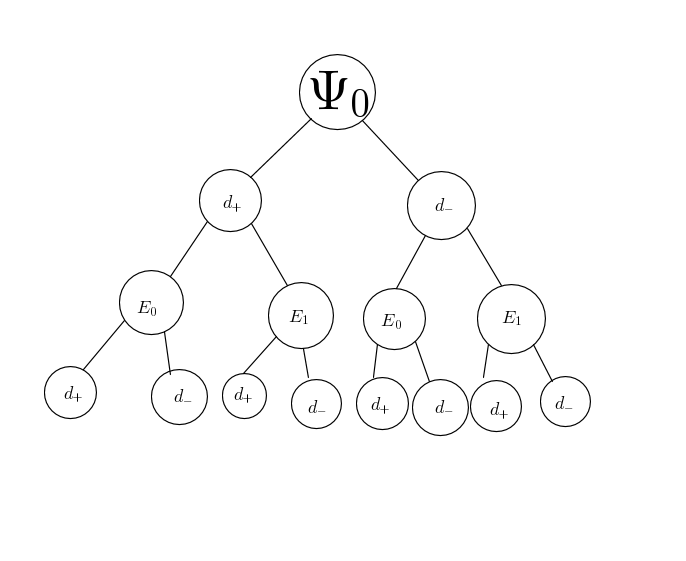
\includegraphics[scale=0.6]{3c.png}
\caption{Et valgtre som viser alle de mulige utfallene vi kan observere.}
\end{figure}

Vi stater med grunntilstanden $\Psi_0$, vi observerer deretter enten $d_+$ eller $d_-$. Bølgelikningen kollapser så til tilstanden som tilsvarer denne målingen ($|d_+\rangle$ eller $|d_-\rangle$). Vi observerer så energien, og måler enten $E_0$ eller $E_1$, og bølgefunksjonen kollapser til forholdsvis $|h_{10}\rangle$ eller $|h_{11}\rangle$. I den lange utregningen under bryter jeg min egen notasjon, og skriver $|E_0\rangle \equiv |h_{10}\rangle $ og $|E_1\rangle \equiv |h_{11}\rangle $, dette er for å gjøre det lettere å lese og skrive, så beklager om dette skaper forvirring, men nå er du advart! Vi gjør så en siste måling og får enten $d_+$ eller $d_-$.\\

Sannsynligheten for å gjøre en viss måling av en tilstand $| f_n\rangle$ når vi har en tilstand $|\psi_n\rangle$ er gitt ved:

$$
|c_n|^2 = |\langle f_n|\psi_n\rangle|^2
$$

(Vi har bare reelle tilstander, så vi kan fjerne $|$ $|$)\\

Sannsynligheten for å måle samme $D$ begge gangene er

\begin{equation}
P(samme) = P(d_+ \cap d_+) + P(d_- \cap d_-)
\label{eq:Psamme}
\end{equation}

Vi finner så at leddene er gitt ved:

$$
P(d_+ \cap d_+) = P(d_+)P(d_+|d_+)
$$

$P(d_+|d_+)$ er sannsynligheten for at vi igjen måler $d_+$ etter vi har målt $d_+$ én gang. Dette er gitt ved sannsynligheten for at vi først måler $E_0$ så $d_+$ eller at vi måler $E_1$ så $d_+$. Så

$$
P(d_+|d_+) = \langle E_0|d_+\rangle^2\langle d_+|E_0\rangle^2 + \langle E_1|d_+\rangle^2\langle d_+|E_1\rangle^2
$$

$\langle E_0|d_+\rangle^2\langle d_+|E_0\rangle^2$ er sannsynligheten for at vi først måler $E_0$ så $d_+$, og $\langle E_1|d_+\rangle^2\langle d_+|E_1\rangle^2$ er sannsynligheten for at vi måler $E_1$ så $d_+$. 

$P(d_+)$ er gitt som:

$$
P(d_+) = \langle d_+|\Psi\rangle^2
$$

For får da:

$$
P(d_+ \cap d_+) = \langle d_+|\Psi\rangle^2\left[\langle E_0|d_+\rangle^2\langle d_+|E_0\rangle^2 + \langle E_1|d_+\rangle^2\langle d_+|E_1\rangle^2\right]
$$


Og helt tilsvarende:

$$
P(d_- \cap d_-) = \langle d_-|\Psi\rangle^2\left[\langle E_0|d_-\rangle^2\langle d_-|E_0\rangle^2 + \langle E_1|d_-\rangle^2\langle d_-|E_1\rangle^2\right]
$$

Vi ender da med at sannsynligheten er:

$$
P(samme) = \langle d_+|\Psi\rangle^2\left[\langle E_0|d_+\rangle^2\langle d_+|E_0\rangle^2 + \langle E_1|d_+\rangle^2\langle d_+|E_1\rangle^2\right] \\
+
 \langle d_-|\Psi\rangle^2\left[\langle E_0|d_-\rangle^2\langle d_-|E_0\rangle^2 + \langle E_1|d_-\rangle^2\langle d_-|E_1\rangle^2\right]
$$

Vi kan så begynne å regne ut dette beistet. Fra tidligere i oppgaven har vi funnet at:

$$
|E_0\rangle = 
\begin{pmatrix}
1\\0
\end{pmatrix}
, \qquad
|E_1\rangle = 
\begin{pmatrix}
0\\1
\end{pmatrix}
$$
$$
|d_+\rangle = 
\frac{1}{\sqrt{4-2\sqrt{2}}}
\begin{pmatrix}
-1+\sqrt{2}\\1
\end{pmatrix}
,\qquad
|d_+\rangle = 
\frac{1}{\sqrt{4+2\sqrt{2}}}
\begin{pmatrix}
-1-\sqrt{2}\\1
\end{pmatrix}
$$
$$
|\Psi(t)\rangle = \frac{1}{\sqrt{5}}
\begin{pmatrix}
2e^{-i(t_D-t_1)} \\ e^{-3i(t_D-t_1)}
\end{pmatrix}
$$

I uttrykket for $|\Psi(t)\rangle$ finner vi en stygg tidsavhengighet, som vi håper vil forsvinne. Vi kan så regne ut indreproduktene:

$$
\langle E_0|d_+\rangle^2 = \left(\frac{-1 + \sqrt{2}}{\sqrt{4-2\sqrt{2}}}\right)^2, \qquad \langle E_0|d_-\rangle^2 = \left(\frac{-1 - \sqrt{2}}{\sqrt{4+2\sqrt{2}}}\right)^2
$$
$$
\langle E_1|d_+\rangle^2 = \frac{1}{4-2\sqrt{2}} ,\qquad \langle E_1|d_-\rangle^2 = \frac{1}{4+2\sqrt{2}} 
$$

Indreprodukt er uavhenging av hvilke vei vi skriver dem, så

$$
\langle d_+|E_0\rangle^2 = \langle E_0|d_+\rangle^2 ,\qquad \langle d_-|E_0\rangle^2 = \langle E_0|d_-\rangle^2
$$
$$
\langle d_+|E_1\rangle^2 = \langle E_1|d_+\rangle^2 ,\qquad \langle d_-|E_1\rangle^2 = \langle E_1|d_-\rangle^2
$$

Vi regner ikke ut $\langle d_{\pm}|\Psi(t)\rangle$ enda, av grunner vi skal se senere! Vi kan nå regne ut leddene i sannsynligheten:

$$
P(d_+ \cap d_+) = \langle d_+|\Psi\rangle^2\left[\langle E_0|d_+\rangle^2\langle d_+|E_0\rangle^2 + \langle E_1|d_+\rangle^2\langle d_+|E_1\rangle^2\right]
$$
$$
= \langle d_+|\Psi\rangle^2\left[\langle E_0|d_+\rangle^2\langle E_0|d_+\rangle^2 + \langle E_1|d_+\rangle^2\langle E_1|d_+\rangle^2\right]
$$
$$
= \langle d_+|\Psi\rangle^2\left[\langle E_0|d_+\rangle^4 + \langle E_1|d_+\rangle^4\right]
$$
$$
= \langle d_+|\Psi\rangle^2\left[\left(\frac{-1+\sqrt{2}}{\sqrt{4-2\sqrt{2}}}\right)^4 + \left(\frac{-1-\sqrt{2}}{\sqrt{4+2\sqrt{2}}}\right)^4\right]
$$
$$
= \frac{3}{4}\langle d_+|\Psi\rangle^2
$$

Og tilsvarende:

$$
P(d_- \cap d_-) = \langle d_-|\Psi\rangle^2\left[\langle E_0|d_-\rangle^2\langle d_-|E_0\rangle^2 + \langle E_1|d_-\rangle^2\langle d_-|E_1\rangle^2\right]
$$
$$
= \langle d_-|\Psi\rangle^2\left[\langle E_0|d_-\rangle^4 + \langle E_1|d_-\rangle^4\right]
$$
$$
= \langle d_-|\Psi\rangle^2\left[ \left(\frac{1}{4-2\sqrt{2}}\right)^2 + \left(\frac{1}{4+2\sqrt{2}}\right)^2\right]
$$
$$
= \frac{3}{4}\langle d_-|\Psi\rangle^2
$$

Og her skjedde det noe utrolig vakkert! Sannsynligheten for at man ved første måling enten finner $d_+$ eller $d_-$ må være $1$. Dette vil si at $\langle d_+|\Psi\rangle^2 + \langle d_-|\Psi\rangle^2 = 1$. Så nå ser vi at:

\begin{equation}
P(samme) = P(d_+ \cap d_+) + P(d_- \cap d_-) = \frac{3}{4}\left(\langle d_+|\Psi\rangle^2 + \langle d_-|\Psi\rangle^2\right) = \underline{\underline{\frac{3}{4}}}
\end{equation}

Siden all tidsavhengighet lå i $\langle d_+|\Psi\rangle$ og $\langle d_-|\Psi\rangle$, og disse forsvant, så betyr det at tidsavhengigheten til sannsynligheten for å finne samme måling begge gangene!\\

Så da har vi funnet at sannsynligheten for å måle samme verdi for $D$ ved to raske målinger er alltid $\underline{\underline{\frac{3}{4}}}$.



\end{document}


